\documentclass{report}
\usepackage[spanish]{babel}
\usepackage[utf8]{inputenc}
\usepackage[T1]{fontenc}
\usepackage{amsthm}
\usepackage{subcaption}
\usepackage{graphicx,wrapfig}
\usepackage{hyperref}
\usepackage[
  top=3cm,
  bottom=3cm,
  left=2cm,
  right=2cm,
  heightrounded,
]{geometry}

\author{
Linares Gil, Daniel
    \thanks{\texttt{daniel.linares@ciencias.unam.mx}\texttt{ - 420490056}}
    \and
García Chavelas, Jonás
    \thanks{\texttt{jonas.garciac@ciencias.unam.mx}\texttt{ - 314152138}}
}
\title{Proyecto 1}
\date{9 de octubre de 2020}

\begin{document}
\maketitle

\section*{Definición del problema}
El aeropuerto de la Ciudad de México nos contrató para una tarea, la cual
es entregar el informe del clima de la ciudad de salida y la ciudad de llegada para 3 mil tickets que
salen el mismo día que se corre el algoritmo. No es interactivo, solo nos interesa el clima \cite{P1}.


\section*{Análisis del problema}
Hay varias dudas que resolver a partir de ésta definición:
\begin{itemize}
\item ¿Importa la fecha de los vuelos? 
\\ No, la definición del problema claramente indica que los tickets salen el mismo día que se corre el algoritmo.
\item ¿Cuál es la entrada del programa?
\\ El programa como tal no tiene entrada, recibe los datos de dos archivos csv que se encuentran en el sistema de archivos.
\item Los vuelos en el \texttt{dataset1} no tienen sitio de origen, ¿cómo procesamos estos vuelos?
\\ Al analizar los datos observamos que estos son vuelos internacionales, así que podemos asumir que saldrán del Aeropuerto Internacional de la Ciudad de México.
\item ¿Qué constituye el clima (variables, descripciones, etc.)?
\\ Las variables que conforman el clima e interesan al cliente son: temperatura máxima, temperatura mínima y humedad. 
\item ¿Qué devuelve el programa?
\\ El programa devuelve información principal del clima (temperatura mínima, máxima, humedad y una descripción general) para las ciudades origen y destino de cada vuelo en la salida estándar, sin ningún formato requerido en particular para la información. 

\end{itemize}
Basado en la información anterior realizamos el análisis inicial del proyecto, en el cual dividimos el problema en dos abstracciones principalmente, una para modelar llamadas a la API de Openweathermap y otra que se encargara de ejecutar el programa que a su vez se dividió en tres subprocesos principales.
\begin{itemize}
    \item Abstracción para la API, esta constituye de un objeto Principal API, que contiene la clave para llamar a la API y provee dos métodos para obtener el clima por coordenadas y por nombre de ciudad, con parámetros auxiliares para escoger el idioma y la unidad de medida de temperatura en la respuesta. Adicional a esto esta abstracción contiene un objeto Clima, el cual es el objeto que se devuelve como resultado de una llamada exitosa a la API y contiene información fundamental del clima (dado que solo era necesaria información principal, muchos datos secundarios de la respuesta son obviados en el diseño de dicho objeto). Además incluimos dos enumeraciones para representar los posibles valores para los parámetros adicionales que requieren los métodos de la API.
    \item Además de esta construimos la abstracción principal del programa. Esta tiene dos objetos, vuelo y ciudad, de modo que un vuelo tiene una ciudad de origen y una de destino, y una ciudad tiene información del nombre,
    coordenadas y el clima, para mantener flexible el programa decidimos permitir ciudades con información incompleta. Además tenemos un objeto App principal, que contiene información sobre la API y controla la lógica principal del proyecto. Dividimos la lógica del objeto App en tres métodos principales:
    \begin{itemize}
        \item Preprocesar los datos: Esta función se encarga de leer el dataset de entrada, identificando de que dataset se trata, y además genera una lista de vuelos y un mapa de nombres de ciudades a ciudades, de modo que mantenemos en nuestra lista de vuelos la información en el mismo orden en que se leyó para ser impresa y evitamos repeticiones en las ciudades para hacer el mínimo de llamadas a la API posibles, ya que las llamadas a la API son la parte más costosa del programa tanto en tiempo como en dinero. Esto último también trae consecuencias negativas, al mantener unicidad en ciudades respecto al nombre, estamos suponiendo que no existen dos ciudades diferentes con el mismo nombre, lo cual en la realidad no es cierto (por ejemplo openweathermap maneja cuatro localizaciones diferentes con el nombre Miami). Sin embargo, consideramos que las ventajas en costo eran suficientes para diseñarlo de esta manera.
        \item Encontrar el clima para las ciudades: Este método recibe el mapa de nombre de ciudades a ciudades y se encarga de buscar el clima para cada ciudad, llamando a los método de la abstracción API por nombre (ya que el cliente nos manifestó su desconfianza en cuanto a la información sobre las coordenadas del  dataset 1, y el dataset 2 no contenía coordenadas). Si se logra encontrar el clima lo almacena en la ciudad y si no lo deja vacío. Además el método se encarga de que no se sobrepase el máximo de llamadas por minuto a la API.
        \item Imprimir el clima: Esta función se encarga de imprimir los resultados del clima para los vuelos, recibiendo la lista de vuelos, e imprimiendo la información en la salida estándar para cada vuelo. Dado que es probable que no se encuentre información sobre el clima para cada ciudad, este método se encarga de manejar estos casos apropiadamente.
    \end{itemize}
\end{itemize}
Luego de esto, nos encontramos con que la API casi no devolvía clima para los datasets. Además prácticamente no encontraba información para el dataset 1 debido a que este contiene códigos IATA de aeropuertos, no nombres de ciudades. Luego de platicarlo con el cliente y conocer su interés porque lográramos encontrar la mayor cantidad de información posible sobre el clima. Decidimos añadir una segunda fase al diseño. \\
En esta fase decidimos desarrollar una base de datos auxiliar en la cual almacenar información sobre ciudades y vuelos, de modo que pudiéramos completar la información de los datasets para así obtener el clima de las ciudades. Para esto obtuvimos la información de todas las ciudades que maneja openweathermap (alrededor de 200,000) en un archivo en formato JSON, así como la información de los aeropuertos en otro archivo JSON. \\
A partir de esto creamos un script para migrar esta información a una base de datos sqlite, la cual consta de dos tablas, una para ciudades y otra para aeropuertos. Estos nos permitió tener un montón de evidencia a partir de la cual deducir de que ciudad preguntar el clima. \\
Además desarrollamos una abstracción para extraer las coordenadas de la ciudad o aeropuerto, para una cadena dada, la cual contó con lo siguiente:
\begin{itemize}
    \item Un objeto principal que al inicializarse abre una conexión a la base de datos y que cuente con un método para obtener coordenadas. Este método recibe una cadena y trata de deducir a que ciudad o aeropuerto se refiere. Para esto normaliza primero la cadena para ampliar las posibilidades de búsqueda y luego busca información en la base de datos en el siguiente orden: Código IATA, Código ICAO, nombre aeropuerto, nombre de ciudad, estado (solo para Estados Unidos) y por último país. Esto con el objetivo de lograr encontrar el clima para la mayor cantidad de vuelos de los datasets. Con esto perdimos especificidad, ya que puede en caso de que se pregunte el clima del país por ejemplo se puede devolver las coordenadas de cualquier ciudad de ese país. Por otro lado al realizar esto logramos reducir el número de llamadas sin resultados a la API a menos de 50, y que todos los vuelos del dataset 1 fueran cubiertos.
    \item Además este modulo tiene un método auxiliar que normaliza cadenas de texto a la forma en la cual se buscan en la base de datos (se remueven todos los caracteres especiales, dejando solamente caracteres alfanuméricos), y decidimos hacer este método publico para que pudiera ser utilizado desde la aplicación principal también, ya que esta también necesita normalizar texto para mantener unicidad en el mapa de nombres de ciudades a ciudades.
\end{itemize}
Por último realizamos los cambios pertinentes para aprovechar esta nueva abstracción en al aplicación principal, modificando lo siguiente:
\begin{itemize}
    \item Preprocesado de datos: En el preprocesado ahora se busca cada ciudad en la base de datos y si se encuentran las coordenadas de esta las define como las encontradas (obviando las que hay en el csv ya que el cliente las consideró poco confiables). En caso de que no se encuentre se intenta buscar en el csv.
    \item Encontrar el clima de las ciudades: En este método ahora se llama a la API primero por las coordenadas en caso  de haber, en caso contrario se intenta por nombre.
\end{itemize}
Además realizamos pruebas unitarias y de integración para asegurar la calidad de nuestra solución.

\section*{Selección de la mejor alternativa}
\begin{itemize}
    \item Paradigma: \\
    El problema al que nos enfrentamos en este proyecto es en principio lineal: \\
    \begin{center}
    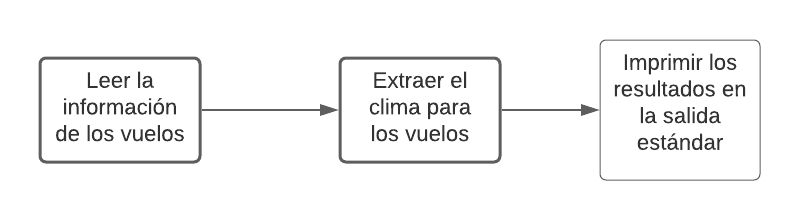
\includegraphics[width=15cm]{images/simple proccess.png}
    \end{center}
    lo cual hace al paradigma imperativo la mejor opción. Unido a esto, muchas de las subtareas del programa se pueden abstraer elegantemente en el paradigma orientado a objetos, por lo cuál este es otro paradigma fundamental para resolver el problema planteado por el cliente. \\
    \item Lenguaje de Programación: \\
    \begin{center}
        
\includegraphics[width=5cm]{images/GOpher.jpg}
    \end{center}
    Para el desarrollo del proyecto decidimos utilizar el lenguaje de programación \href{https://golang.org}{Go}.
    Go es un lenguaje de programación rápido, sencillo, escalable y concurrente desarrollado por Google. Go es imperativo
    y orientado a objetos por lo cual cumple con los paradigmas fundamentales para la resolución del proyecto. Además Go es un lenguaje concurrente que propone un enfoque sencillo y robusto para paralelismo, una de las principales optimizaciones de eficiencia que se pueden desarrollar en el proyecto. Go es un lenguaje desarrollado por Google y utilizado por una amplia variedad de empresas en entornos de producción, por ejemplo, el proyecto \href{https://kubernetes.io}{Kubernetes} está programado en Go. Su uso y soporte por \href{https://brainhub.eu/blog/biggest-companies-using-golang/}{grandes empresas}, junto con su creciente popularidad, hacen de Go un lenguaje a prueba del tiempo, lo cual otorga al proyecto estabilidad a largo plazo. Go es utilizado principalmente para \href{https://eng.uber.com/go-geofence-highest-query-per-second-service/}{programas que necesitan hacer una tarea, y necesitan hacerla bien}, el proyecto entra en esta definición, lo cual hace a Go una muy buena alternativa para su implementación. \\\\
    Sin embargo, Go no fue el único lenguaje que tuvimos en cuenta para implementar nuestra solución, a continuación se encuentran las principales alternativas que tuvimos en cuenta, y las razones por las cuales preferimos Go a estas.
    \begin{itemize}
        \item \textbf{\href{https://www.scala-lang.org/}{Scala}}: Scala es un lenguaje multiparadigma poderoso que aprovecha la JVM de Java para tener acceso a todas sus bibliotecas, pero su complejidad hizo que acabaramos prefiriendo Go a este.
        \item \textbf{\href{https://python.org}{Python}}: Python es sin duda una gran elección para cualquier proyecto de software hoy en día, pero el tipado estático y la simpleza de Go, hicieron que nos decantáramos por este.
    \end{itemize}
    \item API utlilizada: Utilizamos la API de \href{https://openweathermap.org/current}{openweathermap} principalmente por su buena documentación y porque el cliente nos la recomendó.
    \item Servidor de Base de Datos utilizado: Utilizamos \href{https://www.sqlite.org/index.html}{sqlite} principalmente porque la base de datos es solo un archivo y no necesita configuración en la maquina que ejecuta el programa.
    \item Bibliotecas de terceros: \\
    Para el desarrollo de la solución requerimos varias bibliotecas, principalmente parte de la biblioteca estándar del lenguaje, las cuales se muestran a continuación:
    \begin{itemize}
        \item \href{https://golang.org/pkg/encoding/json/}{\texttt{enconding/json}}: Utilizamos este paquete para decodificar la respuesta de la API en formato json a una estructura de Go.
        \item \href{https://golang.org/pkg/encoding/csv/}{\texttt{enconding/csv}}: Utilizamos este paquete para leer los archivos de entrada en formato csv.
        \item \href{https://golang.org/pkg/fmt/}{\texttt{fmt}}: Paquete útil para imprimir y formar cadenas de texto.
        \item \href{https://golang.org/pkg/strconv/}{\texttt{strconv}}: Fue útil para convertir cadenas a tipos númericos.
        \item \href{https://golang.org/pkg/strings/}{\texttt{strings}}: Útil para procesar cadenas como por ejemplo, convertir los caracteres  de una cadena a mayúsculas.
        \item \href{https://golang.org/pkg/unicode/}{\texttt{unicode}}: Provee tipos útiles para manejar clases de caracteres en formato unicode. Usado principalmente para remover caracteres especiales a la hora de normalizar cadenas.
        \item \href{https://golang.org/pkg/os/}{\texttt{os}}: Lo utilizamos principalmente para acrir archivos del sistema, tanto los datasets de entrada como el archivo de la base de datos.
        \item \href{https://golang.org/pkg/time/}{\texttt{time}}: Lo utilizamos para manejar el tiempo de espera de un minuto cada 60 queries a la API y para el tiempo de espera máximo permitido para una llamada a la API.
        \item \href{https://golang.org/pkg/errors/}{\texttt{errors}}: Lo utilizamos para crear errores en caso de que algo no ocurriera como previsto.
        \item \href{https://golang.org/pkg/net/http/}{\texttt{net/http}}: Utilizamos el paquete para realizar las llamadas a la API de openweathermap.
        \item \href{https://golang.org/pkg/database/sql/}{\texttt{database/sql}}: Utilizamos el paquete para conectarnos a la base de datos.
    \end{itemize}
    También requerimos algunos paquetes de terceros, principalmente por dos razones:
    \begin{itemize}
        \item \href{https://github.com/mattn/go-sqlite3/}{\texttt{go-sqlite3}}: Driver para conectarse a sqlite-3, el servicio de base de datos utilizado en el programa.
        \item \href{https://golang.org/x/text/runes/}{\texttt{runes}}, \href{https://golang.org/x/text/transform/}{\texttt{transform}},
        \href{https://golang.org/x/text/unicode/norm/}{\texttt{norm}}: Estos tres paquetes fueron utilizados para normalizar el texto y removerle acentos.
    \end{itemize}
\end{itemize}

\section*{Diagrama de flujo}
Dado que los archivos de entrada se encuentran dentro del mismo sistema usando el programa sólo necesitamos leer el texto para extraer la información relevante, que en éste caso son las ciudades de origen y destino; podemos unir ambas cosas como una estructura que denominaremos como el vuelo, luego cada ciudad tiene su propio nombre, coordenadas y clima, que es la variable que realmente nos interesa y que dejaremos como \texttt{NIL} por ahora, ya que no tiene caso definirla aún. Durante todo esto debemos tener en cuenta los posibles errores que pudiera haber en los datos que estamos a punto de almacenar, así podemos descartar o corregir cualquiera de estos.\\Para reducir el número de requests que hacemos a la API y al mismo tiempo almacenar las ciudades, pretendimos usar un conjunto de ciudades, después se hace la request de cada ciudad, con lo que el clima debería quedar definido para cada vuelo. \\Finalmente debemos asegurarnos de no pasarnos del límite de requests que permite la API, por lo que habrá que esperar (en el caso de openweathermap un minuto) para poder recibir todos los climas, una vez hecho esto basta con imprimir los datos relevantes que conforman los vuelos en la terminal.

\begin{center}
    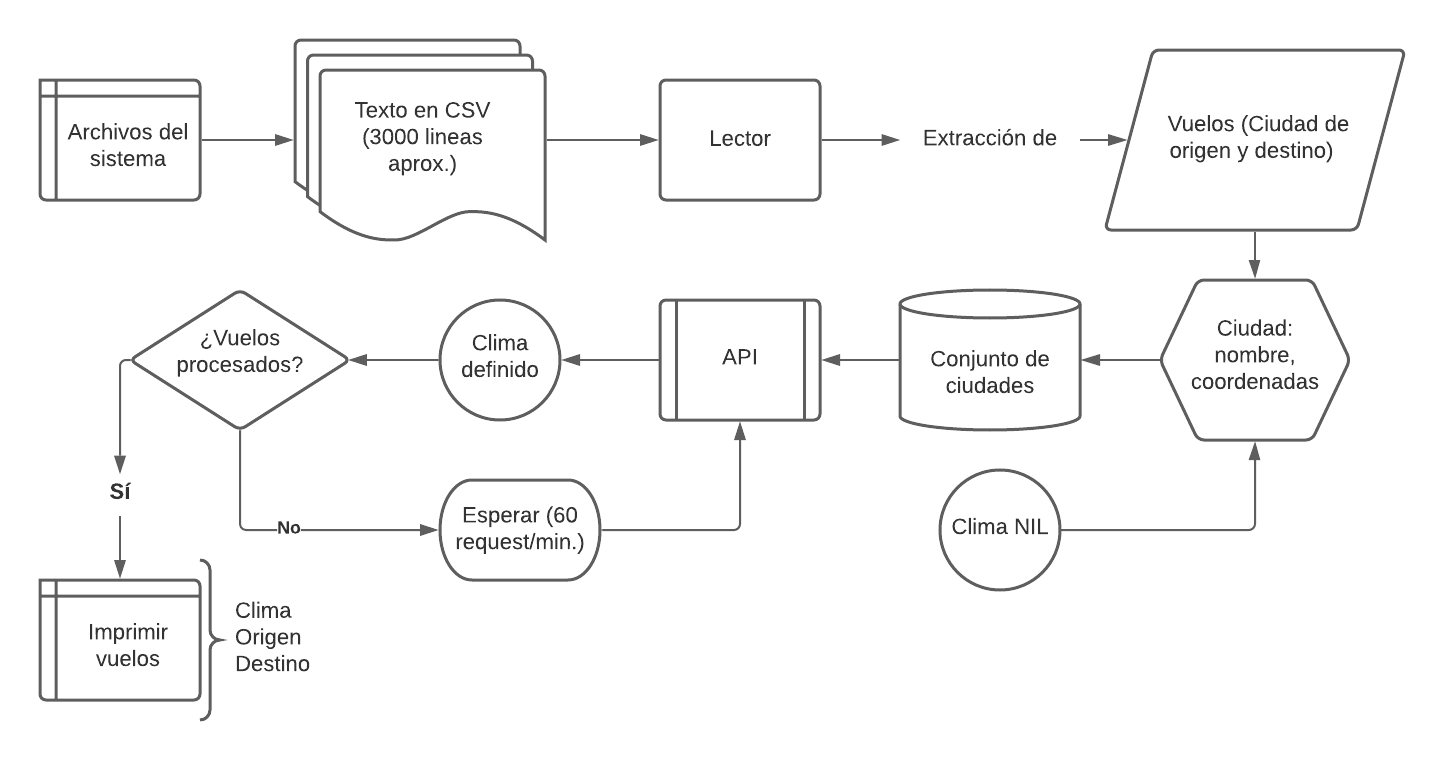
\includegraphics[width=17cm]{images/flow.png}
\end{center}

\section*{Mantenimiento}
El programa puede requerir mantenimiento en diversas áreas entre las cuales se encuentran:
\begin{itemize}
    \item Corrección de errores.
    \item Mantenimiento de la base de datos, ya sea para añadir ciudades o aeropuertos a ésta.
    \item En caso de cambios en la API de openweathermap.
\end{itemize}
\subsection*{Posibles mejoras}
Proponemos las siguientes mejoras para el programa:
\begin{itemize}
    \item Hacerlo concurrente: Una de las principales mejoras en la eficiencia es hacer las llamadas a la API de manera concurrente en vez de secuencialmente.
    \item Convertir el programa en un micro-servicio: El programa podría ser adaptado para funcionar como un servicio en la nube y así poder extender su uso a todos los aeropuertos de México, así como para proveer el clima a aplicaciones web de aeropuertos y aerolíneas.
    \item Guardar la cache y la información del clima en un almacenamiento persistente: Actualmente el programa guarda la información que procesa solamente en memoria, por lo que en caso de una falla de hardware esta se podría perder y sería necesario reiniciar el proceso. Al hacer el programa persistente se se podría recuperar el estado en el que se encontraba el programa antes antes de que ocurriera la falla, lo cual provee al programa una mayor robustez.
\end{itemize}

\subsection*{Presupuesto}
Tomando en cuenta que: 
\begin{itemize}
    \item Se hizo programa que nos devuelve el clima de las ciudades de origen y destino de varios vuelos.
    \item Y la cantidad de tiempo empleado (alrededor de cincuenta horas empleadas por el equipo).
\end{itemize}

Consideramos adecuado un pago de \texttt{\$20,000.00}.
\\ \\
Adicionalmente se cobrará \texttt{\$1,200.00} por ocho horas de trabajo el mantenimiento en el programa, mientras que el costo de las mejoras dependerá de las mismas y los recursos empleados para hacerlas.
\bibliographystyle{plain}
\bibliography{refs}

\end{document}